\byline{{\textbf{\Large\sffamily October Bonsai Club Meetup:}}\\
        {\textbf{\large\sffamily Not Even Storm Amy Could Blow Us Away!}}}{The Newsletter Team}
\vspace*{-0.75em}
\noindent
Despite the blustery winds and rains brought by Storm Amy, our club evening went ahead in true bonsai spirit --- calm, steady, and deeply rooted!
More than twenty members gathered at the Whitton Community Centre, with a wonderful mix of familiar faces and a few new ones joining our growing family of enthusiasts.

This month's meeting stood out for its open, hands\--on atmosphere.
With no formal workshop scheduled, members were invited to bring along their own trees to work on throughout the evening.
The result was a lively exchange of ideas, techniques, and laughter.
Seasoned members offered thoughtful feedback and guidance, while newcomers absorbed valuable lessons --- insights they'll no doubt carry with them as they continue their bonsai journey.
% 
The evening followed closely on the heels of the \textbf{Heathrow Bonsai Show}, and conversations buzzed with stories from the event.
Those who attended shared highlights, impressions, and even a little friendly bragging about their latest acquisitions!
For anyone who couldn't make it to the show, don't worry --- we've prepared a feature inside this issue with photos and a full report.
%
Of course, no club night would be complete without our \textbf{Tree of the Month} competition.
October's theme, \textit{``Autumn Colours, Any Tree,''} inspired a stunning array of entries.
Both our newer and long\--standing members rose to the occasion, presenting trees ablaze with the fiery hues of the season.
Turn the page to see which displays captured admiration this month.

Looking ahead, November promises two important dates.
On \textbf{Thursday 13th November}, we'll hold our \textbf{Annual General Meeting (AGM)} in the Trimble Lounge.
Later, on \textbf{Thursday 27th November}, we welcome \textbf{David Cheshire} for a demonstration and talk --- an evening not to be missed! The \textbf{Tree of the Month} theme will be \textit{``Any Tree Previously Submitted During the Year.''} See you all there for another month of learning and inspiration.

\begin{window}[%
    2,l,%
    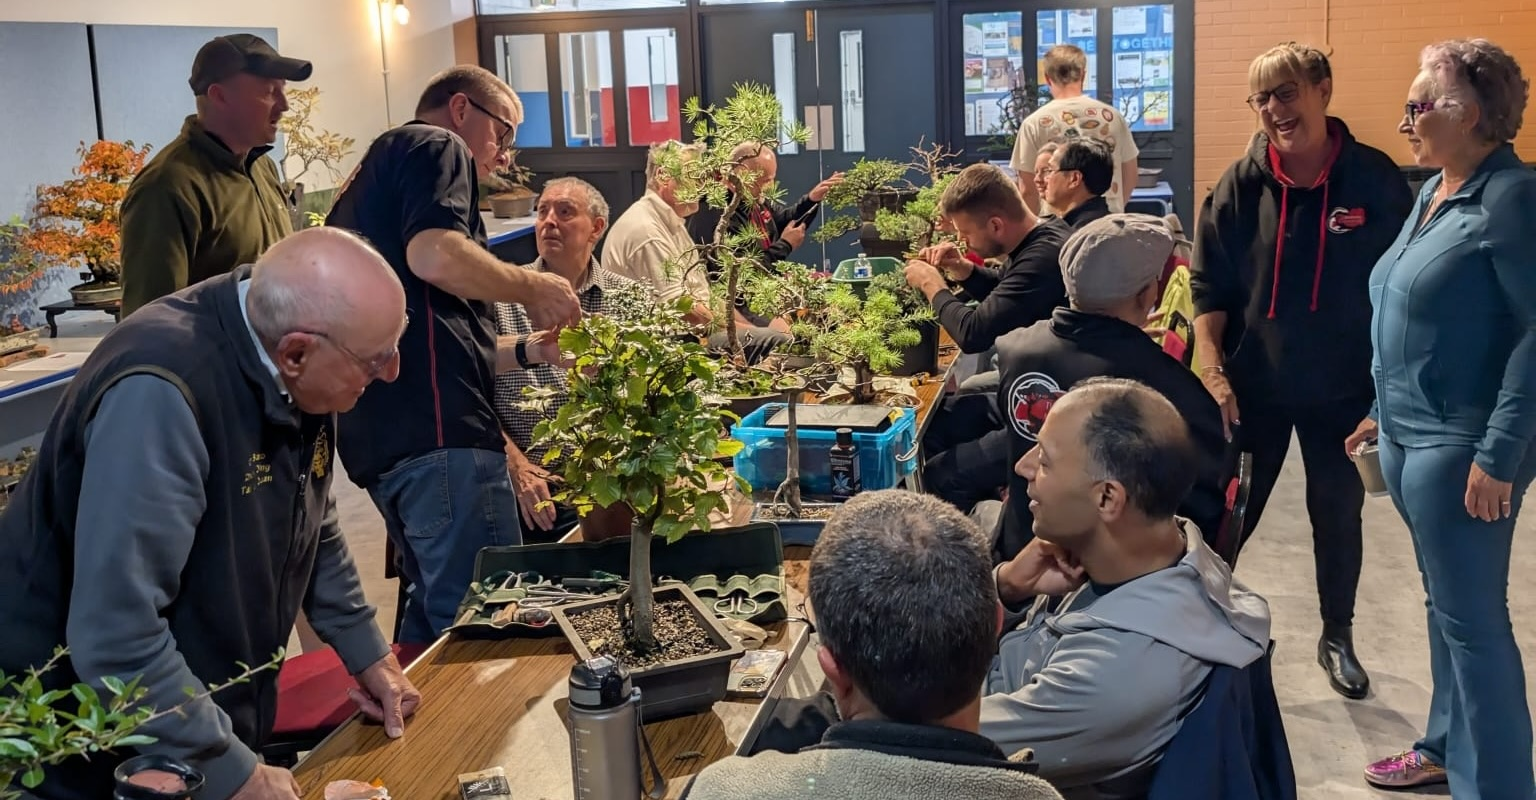
\includegraphics[width=1.0\columnwidth]{2025_10/res/editorial_october},%
    \centerline{\emph{Members sharing techniques during October's open workshop evening.}}%
]
\end{window}
\closearticle
\clearpage
